%\documentclass[aps,prl,groupedaddress]{revtex4-1}  % One column - tight
%\documentclass[aps,prl,preprint,groupedaddress]{revtex4-1}  % One column - spread
\documentclass[aps,prl,reprint,groupedaddress]{revtex4-1}  % Two column
%\documentclass[aps,prl,preprint,superscriptaddress]{revtex4-1}
%\documentclass[aps,prl,reprint,groupedaddress]{revtex4-1}

% Use the \preprint command to place your local institutional report
% number in the upper righthand corner of the title page in preprint mode.
% Multiple \preprint commands are allowed.
% Use the 'preprintnumbers' class option to override journal defaults
% to display numbers if necessary
%\preprint{}

% You should use BibTeX and apsrev.bst for references
% Choosing a journal automatically selects the correct APS
% BibTeX style file (bst file), so only uncomment the line
% below if necessary.
%\bibliographystyle{apsrev4-1}

% % % % % % % % % % % % Noam% % % % % % % % % % % % 
% Added preamble commands:
\usepackage[utf8]{inputenc}
\usepackage{array}
\usepackage{mathrsfs}
\usepackage{multirow}
\usepackage{amsmath}
\usepackage{graphicx}
\usepackage{float}  % For forcing a float position using 'H'.
\graphicspath{{../../figures/}}  % Search for graphics within the given directories.
\usepackage[unicode=true,pdfusetitle,bookmarks=true,bookmarksnumbered=false,bookmarksopen=false,
 breaklinks=false,pdfborder={0 0 1},backref=false,colorlinks=false]{hyperref}
%%%%%%%%%%%%%%%%%%%%%%%%%%%%%% User specified LaTeX commands.
\usepackage{braket}
\hypersetup{colorlinks=True,urlcolor=blue,linkcolor=blue,citecolor=blue,filecolor=black}
\usepackage[caption=false]{subfig}
% Extra commands
%\usepackage{lmodern}
%\usepackage[T1]{fontenc}
%\setcounter{secnumdepth}{3}
%\usepackage{color}
%\usepackage{float}
%\usepackage{mathtools}
%\usepackage{amssymb}
%\usepackage{breakurl}

%\usepackage{pslatex}  % Change font style.
%\renewcommand{\arraystretch}{1.5}  % Widens rows in Tables
%\setlength{\extrarowheight}{2pt}   % Widens rows in Tables

\makeatletter

\makeatother

\begin{document}

%Title of paper
\title{Final Project - TALENT 2017 at ECT*}

% repeat the \author .. \affiliation  etc. as needed
% \email, \thanks, \homepage, \altaffiliation all apply to the current
% author. Explanatory text should go in the []'s, actual e-mail
% address or url should go in the {}'s for \email and \homepage.
% Please use the appropriate macro foreach each type of information

% \affiliation command applies to all authors since the last
% \affiliation command. The \affiliation command should follow the
% other information
% \affiliation can be followed by \email, \homepage, \thanks as well.
\author{N. Gavrielov}
%\email[]{Your e-mail address}
%\homepage[]{Your web page}
%\thanks{}
%\altaffiliation{}
\affiliation{}

%Collaboration name if desired (requires use of superscriptaddress
%option in \documentclass). \noaffiliation is required (may also be
%used with the \author command).
%\collaboration can be followed by \email, \homepage, \thanks as well.
%\collaboration{}
%\noaffiliation

\date{\today}

\begin{abstract}
% insert abstract here
\end{abstract}

% insert suggested PACS numbers in braces on next line
\pacs{}
% insert suggested keywords - APS authors don't need to do this
%\keywords{}

%\maketitle must follow title, authors, abstract, \pacs, and \keywords
\maketitle


\section{Introduction of our Theoretical Framework}

The oxygen isotopes have been widely investigated \citep[for a review see][]{Brown2017}. To describe their low lying spectrum within the shell model, different model spaces and interactions are used, starting from an $^{16}$O core with extra neutrons in the $sd$-shell \cite{Kuo1966,Wildenthal1984,Brown1988,Brown2006}, adding the lower $p$-shell for core-excitation (intruder states) with particle-hole configurations \cite{Lawson1976} and incorporating the $pf$-shell as well \cite{Utsuno1999}.

In this work we investigate the structural changes of the $^{18-28}$O isotopes, both even and odd, by examining their low-lying states. This is done by developing our own shell model program and comparing the energies it generates with different effective interactions using NushellX@MSU program \cite{Brown2014}. Further work includes using NushellX@MSU to calculate $E2$ transition rate and Fermi and Gamow-Teller $\beta$-decay.

We use an $^{16}$O core, having 8 protons and 8 neutron at the $s$-$p$-shells, ($0s_{1/2},0p_{3/2},0p_{1/2}$). 
More neutrons are then excited in the $sd$-shell ($0d_{5/2},1s_{1/2},0d_{3/2}$), which serves as our model space. We use all possible configurations in these orbits and work in a harmonic oscillator basis with spin-orbit splitting. 
The Hamiltonian reads

		\begin{equation} \label{eq:H}
		\hat H = \hat H_0 + \hat H_I,
		\end{equation}
for
		\begin{equation} \label{eq:H_0}
		\hat H_0 = \sum_{p,q} \epsilon_p \hat a_{p}^\dagger \hat a_{q},
		\end{equation}
the one-body Hamiltonian, where $\hat n_p = \hat a_p^\dagger \hat a_p$ is the number operator for the spherical orbit $p$ with quantum numbers ($n_p,\ell_p,j_p,m_p$) and $\epsilon_p = \braket{p|h_0|p}$ are the single-particle energies (SPE). The interaction part reads
		\begin{equation} \label{eq:V}
		\hat H_I = \sum_{p < q=1}^{N} \sum_{r < s=1}^{N} V(p,q;r,s) \hat T(p,q;r,s),
		\end{equation}
		with
		\begin{equation} \label{eq:P}
		\hat T(p,q;r,s)  = \hat P_{p,q}^+ \hat P_{r,s}^-,
		\end{equation}
where $\hat P_{p,q}^+ = \sum_{p,q} \hat a_p^\dagger \hat a_q^\dagger, \qquad
								  \hat P_{r,s}^- = \sum_{r,s} \hat a_r \hat a_s.$

$\hat H_I$ is given in $M$-scheme and is the two-body density operator for nucleon pairs in orbits $p,q$ and $r,s$ coupled to the total spin projection $M$, where $N$ is the number of particles in the configuration. In $J$-scheme $\hat H_I$ reads 
\begin{equation}
	\hat H_I =  \sum_{a\leq b,c \leq d} \sum_{JT} V_{J,T}(p,q;r,s) \hat T_{J,T}(p,q;r,s),
\end{equation}
where $\hat T_{J,T}(p,q;r,s)$ is the scalar two-body density operator for nucleon pairs in orbits $p,q$ and $r,s$ coupled to spin quantum numbers $J,M$ and isospin quantum numbers $T,T_z$ \cite{Brown2006}. Here the appropriate quantum numbers are $(n_i,\ell_i,j_i)$, $i \in \{a,b,c,d\}$. The transformation between the two-body matrix elements (TBME) from $J$- to $M$-scheme reads
\begin{align}
	\nonumber
	V(p,q;r,s) & =  \braket{j_{p},m_{p};j_{q},m_{q}|V|j_{r},m_{r};j_{s},m_{s}} \\ \nonumber
			   & =  \sum_{J,M} \braket{j_{p},m_{p};j_{q},m_{q}|JM} \braket{j_{r},m_{r};j_{s},m_{s}|JM} \\
			   &	\times \braket{(j_{p},j_{q})JM|V|(j_{r},j_{s})JM},
\end{align}
where $\braket{j_{a},m_{a};j_{b},m_{b}|JM}$ is a Clebsch-Gordan coefficient and other quantum numbers are implicitly implied.

We use the SPE and TBME of the USDB interaction \cite{Brown2006} and work in $M$-scheme. The SPE values and order is given in Table \ref{tab:SPE}. The TBME for $A=18$ are given in \cite{Brown2006} in $J$-scheme for $T=1,0$ in Tables I and II, respectively. As was done for the USD interaction \cite{Wildenthal1984}, the SPE are taken to be mass independent and for the TBME we employ a mass dependence of the form
\begin{equation}
	V(p,q;r,s)(A) = \left( \frac{18}{A} \right)^p V(p,q;r,s)(A=18),
\end{equation}
with $p=0.3$. This qualitative mass dependence is expected from the evaluation of a medium-range interaction with harmonic-oscillator radial wave functions. It also defines TBME for other $A$ values in the $sd$-shell.

Using the single-particle states (SPS) we construct the appropriate slater determinants according to the number of particles which we place in the $sd$-shell. This enables us to construct expectation values of the Hamiltonian \eqref{eq:H} and diagonaliz it to obtain the energies. 

\begin{table}[H]
\caption{Single particle energies of the $sd$-shell in the $M$-scheme basis with their corresponding quantum numbers: $N$, the principle quantum number; $\ell$, the orbital angular momentum; $J$, the total angular momentum; $M_j$, the total angular momentum projection on the $z$ axis. \label{tab:SPE}}
\begin{ruledtabular}
\begin{tabular}{c|cccccc}
index	&	$N$	&	$\ell$	&	$J$	&	$M_j$	&	SPE			\\
\hline 
1		&	1	&	0		&	1	&	$-1/2$	&	-3.20790	\\
2		&	1	&	0		&	1	&	$+1/2$	&	-3.20790	\\
3		& 	0	&	2		&	3	&	$-3/2$	&	 2.11170	\\
4		&	0	&	2		&	3	&	$-1/2$	&	 2.11170	\\
5		&	0	&	2		&	3	&	$+1/2$	&	 2.11170	\\
6		&	0	&	2		&	3	&	$+3/2$	&	 2.11170	\\
7		&	0	&	2		&	5	&	$-5/2$	&	-3.92570	\\
8		&	0	&	2		&	5	&	$-3/2$	&	-3.92570	\\
9		&	0	&	2		&	5	&	$-1/2$	&	-3.92570	\\
10		&	0	&	2		&	5	&	$+1/2$	&	-3.92570	\\
11		&	0	&	2		&	5	&	$+3/2$	&	-3.92570	\\
12		&	0	&	2		&	5	&	$+5/2$	&	-3.92570	
\end{tabular}
\end{ruledtabular}
\end{table}

\section{Structure of the Oxygen Isotopes}
The structure of the wave functions of different levels in these isotopes is interesting to examine since they can reveal the role of different configurations and orbits. Furthermore, within a given configuration examining different interactions using different observables can be also insightful. Thus one can examine, on top of low lying energies, electromagnetic transitions rates. Here we will only investigate the $E2$ between the first $2^+$ and the first $0^+$, i.e. $B(E2; 2_1^+ \rightarrow 0_1^+)$, using the USDA, USDB and CCEI interactions in NushellX@MSU, given in Fig. \ref{oxygen-be2}. For the experimental data there are only three values, however it is notable that they become closer to the theoretical values as neutrons are added, with the largest discrepancy occurring for the $^{18}$O isotope. The reason might be due to the fact we are neglecting $p$-shell core-excitations when using only the $sd$-shel model space. It was found in \cite{Lawson1976} that the $0_2^+$ should have a dominant $4p-2h$ component. However there are indications that larger mixing with the $0_1^+$ should arise. The problem for mixing of these states due to the truncation in the $np–mh$ sequence is discussed in \cite{Warburton1992a}. Therefore, when close to the $^{16}$O core, e.g. at $^{18}$O, a large part of the $p$-shell is missing in the wave function rendering less components in the wave functions to connect between the $0_1^+$ and the $2_1^+$ and hence yielding a smaller $B(E2)$ value. As neutrons are added to the $^{16} $O core, the $p$-shell core-excitations move to higher energy and mix less with the low-lying states, then the $sd$-shell model space becomes a better approximation. As seen in Fig. \ref{oxygen-be2}, this is correct for all three interactions which operate in the $sd$-shell. Although the CCEI does not reproduce energies as well as USDA and USDB, it gives a slightly better approximation for the $B(E2; 2_1^+ \rightarrow 0_1^+)$. Yet, the differences are minor and other observables should be examined.

\begin{figure}[h]
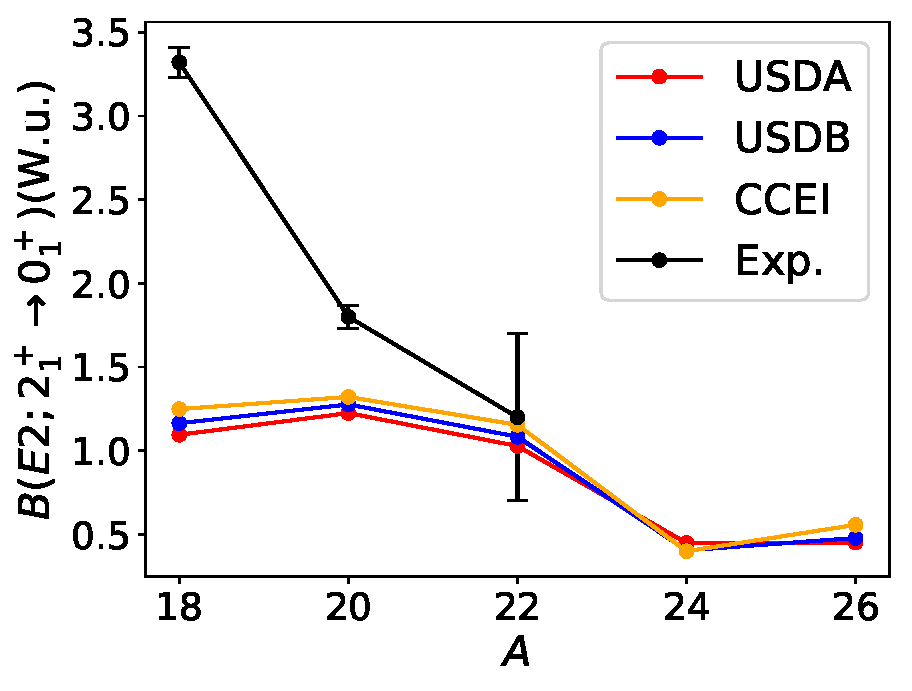
\includegraphics[width=1\linewidth]{../figures/oxygen-be2.pdf}
\caption{$B(E2; 2^+ \rightarrow 0^+)$ of experimental (black), the USDA (red), USDB (blue) and CCEI (orange) interactions for $^{18-26}$O. \label{oxygen-be2}}
\end{figure}

\pagebreak
\bibliography{noam.bib}
\end{document}


